\section{C++性能优化实践}
\label{sec:cpp_optimization}

\subsection{背景}

游戏引擎对性能有着极高的要求：每帧需要在16毫秒内完成所有逻辑和渲染。C++作为系统级编程语言，提供了丰富的性能优化手段。本项目充分利用C++20标准和现代编译器优化技术，在保证代码可维护性的同时实现高性能。

\subsection{编译器配置}

\subsubsection{C++标准与编译选项}

项目采用C++20标准，禁用编译器扩展以保持标准兼容性。针对不同编译器配置了专门的优化选项：

\textbf{MSVC (Windows)}优化选项：
\begin{itemize}
    \item \texttt{/O2}：最大化速度优化
    \item \texttt{/arch:AVX2}：启用AVX2指令集，利用现代CPU的SIMD能力
    \item \texttt{/fp:fast}：快速浮点数模型，允许编译器重排浮点运算
    \item \texttt{/Oi}：启用内联函数优化
    \item \texttt{/LTCG}：全程序优化，跨编译单元内联
    \item \texttt{/OPT:REF,ICF}：移除未引用代码，合并相同函数
\end{itemize}

\textbf{GCC/Clang (Linux/macOS)}优化选项：
\begin{itemize}
    \item \texttt{-O3}：最高优化等级，启用所有-O2优化加额外激进优化
    \item \texttt{-march=native -mtune=native}：针对本地CPU架构优化，生成特定指令
    \item \texttt{-ffast-math}：快速数学运算，允许不严格的IEEE浮点语义
    \item \texttt{-fno-trapping-math}：禁用浮点异常陷阱
\end{itemize}

\subsubsection{警告配置}

项目配置了严格的编译器警告，并将关键警告视为错误：

\begin{itemize}
    \item MSVC：\texttt{/W4}（高警告级别），\texttt{/we4172}（返回局部变量地址）、\texttt{/we4701}（使用未初始化变量）等视为错误
    \item GCC/Clang：\texttt{-Wall -Wextra -Wpedantic}，\texttt{-Werror=return-local-addr}、\texttt{-Werror=uninitialized}等视为错误
\end{itemize}

所有编译警告必须解决，确保代码质量。

\subsection{C++20特性应用}

\subsubsection{if constexpr编译期分支}

项目中大量使用\texttt{if constexpr}进行编译期分支选择，共35+处。编译器会在编译时决定执行哪个分支，消除运行时开销：

典型应用场景包括处理不同函数返回类型（void与非void）、根据类型大小选择序列化方式、针对特定类型启用特殊功能。这种方式避免了虚函数调用和运行时类型检查。

\subsubsection{std::optional可选值}

项目广泛使用\texttt{std::optional}处理可能缺失的值，共367处。相比传统的指针或错误码，\texttt{std::optional}更加类型安全，避免了空指针解引用风险。

\subsubsection{[[nodiscard]]属性}

项目有10000+处使用\texttt{[[nodiscard]]}属性，确保返回值不被忽略。这对于\texttt{Result<T>}类型尤其重要，防止错误处理被遗漏。

\subsubsection{constexpr编译期计算}

项目有2926+处使用\texttt{constexpr}，主要包括：

\textbf{编译期常量}：游戏常量（如TICK\_DURATION\_MS = 50）、数学常量（PI、E等）、配置参数（PICKUP\_RANGE = 1.0f等）。

\textbf{编译期函数}：数学函数（toRadians、toDegrees、clamp、square）、类型萃取辅助函数。

编译期计算将运行时开销转移到编译时，同时确保常量表达式的正确性。

\subsection{内存管理策略}

\subsubsection{智能指针体系}

项目建立了完整的智能指针使用规范：

\textbf{unique\_ptr独占所有权}：大多数资源（World、ChunkManager、PhysicsEngine、LightManager等）使用\texttt{std::unique\_ptr}管理，确保资源生命周期明确。

\textbf{shared\_ptr共享所有权}：异步场景（如跨线程共享的ChunkData、取消令牌）使用\texttt{std::shared\_ptr}，配合\texttt{std::weak\_ptr}避免循环引用。

\textbf{手动new/delete极少}：全项目仅367处手动内存管理，智能指针覆盖率极高。

\subsubsection{容器优化}

项目有440处使用容器优化方法：

\textbf{reserve预分配}：在知道容器最终大小时预分配容量，避免多次重新分配。例如，区块网格生成前预分配顶点和索引缓冲区。

\textbf{emplace原地构造}：使用\texttt{emplace\_back}/\texttt{emplace}避免临时对象构造和移动。

\textbf{shrink\_to\_fit}：释放多余容量，减少内存占用。

\subsubsection{方块状态系统紧凑化}

\textbf{背景：什么是方块状态？}

在Minecraft中，方块不仅仅是简单的ID。以熔炉为例，它同时具有方向属性和燃烧状态：
\begin{itemize}
    \item \texttt{facing}：朝向（NORTH、SOUTH、EAST、WEST共4个值）
    \item \texttt{lit}：是否点燃（false、true共2个值）
\end{itemize}

这两种属性的合法组合共有$4 \times 2 = 8$种，每种组合都是一个独立的\texttt{BlockState}对象。类似地，木门有$2^3 = 8$种状态（开关、铰链位置、上下半），而栅栏的连接状态组合可能多达数十种。Minecraft在启动时会预生成所有方块的所有状态组合——假设有800个方块，平均每个方块20个状态，就是约16000个状态对象。

\textbf{状态空间的多维数组视角}：若将方块的属性空间视为多维离散坐标，则所有状态可以映射到一维数组。以熔炉为例，其8种状态可排列为$2 \times 4$的矩阵，如图\ref{fig:state_matrix}所示。

\begin{figure}[h]
\centering
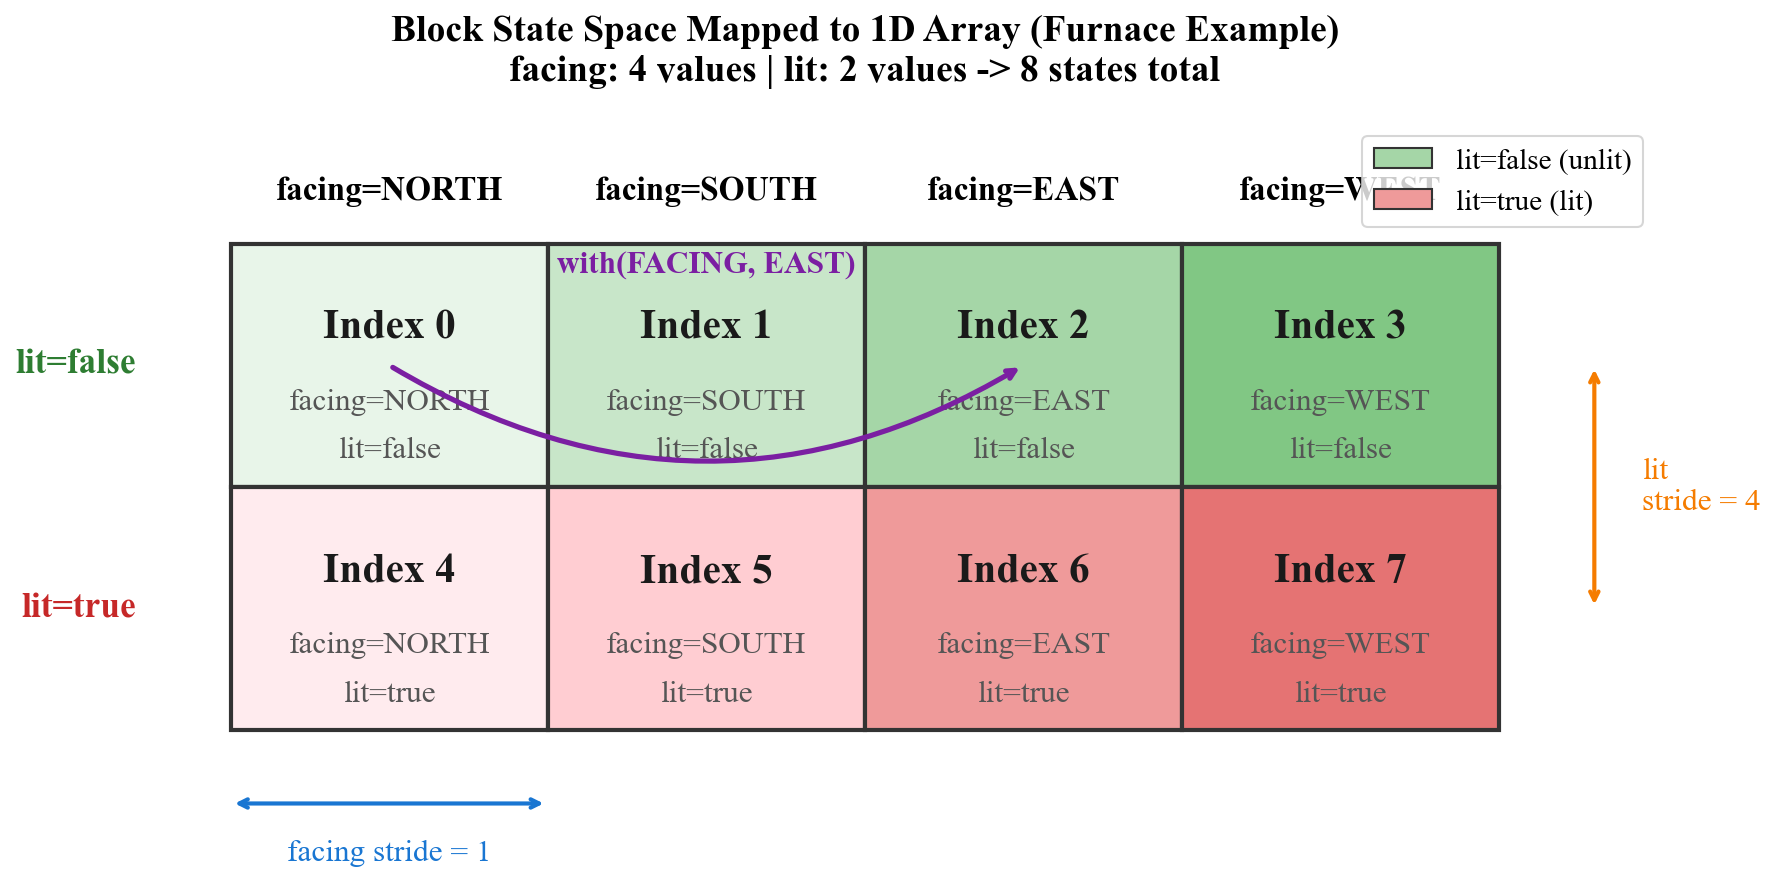
\includegraphics[width=0.95\linewidth]{images/state_matrix.png}
\caption{方块状态空间映射为一维数组示意图。以熔炉为例，\texttt{facing}有4个值、\texttt{lit}有2个值，共8种状态。左侧两行为不同\texttt{lit}值对应的状态，顶部四列为不同\texttt{facing}值对应的状态。每个单元格内的数字为该状态在一维数组中的索引。图中展示了\texttt{with(FACING, EAST)}操作如何通过步长计算实现O(1)状态切换。}
\label{fig:state_matrix}
\end{figure}

图中关键概念说明：
\begin{itemize}
    \item \textbf{步长（stride）}：某属性变化时，状态索引的增量。\texttt{facing}的步长为1（相邻状态仅\texttt{facing}不同），\texttt{lit}的步长为4（跨过所有\texttt{facing}值才变\texttt{lit}）
    \item \textbf{索引计算}：\texttt{stateIndex = facing\_index × 1 + lit\_index × 4}
    \item \textbf{状态切换}：\texttt{targetIndex = currentIndex + (targetValue - currentValue) × stride}，纯整数运算即可定位目标状态
\end{itemize}

Minecraft中的\texttt{BlockState}和\texttt{FluidState}是典型的高频小对象：方块注册时会为每个方块预生成所有合法状态组合，后续世界存储、渲染、命令解析、结构放置、掉落表匹配等系统都频繁访问这些状态。如果每个状态都额外持有多张哈希表，则会显著放大内存占用，并降低缓存局部性。

\textbf{原始设计问题}：项目早期的\texttt{StateHolder}为每个状态保存两类动态结构：
\begin{itemize}
    \item \texttt{unordered\_map<const IProperty*, size\_t>}：记录每个属性当前取值的索引
    \item \texttt{unordered\_map<const IProperty*, vector<const State*>>}：记录\texttt{with()}状态切换的跳转表
\end{itemize}

这种设计虽然接口直接，但存在两个明显缺陷。第一，每个状态对象都重复保存属性键和值，形成较大的对象图和额外的堆分配。第二，\texttt{StateContainer}在构建时需要枚举所有状态，并对每个属性值组合做匹配查找，构建复杂度较高。

\textbf{优化后的布局}：本项目将状态系统改为“容器持有元数据，状态持有紧凑索引”的方案：
\begin{itemize}
    \item 每个\texttt{StateContainer}保存属性布局表（属性指针、槽位索引、stride）
    \item 每个具体状态仅保存\texttt{vector<size\_t>}形式的属性值索引数组
    \item \texttt{with()}不再查哈希表，而是通过当前状态在线性布局中的索引和属性stride直接计算目标状态位置
\end{itemize}

\textbf{核心思想}：若一个方块的属性空间可表示为多维离散坐标，则所有状态可以按行主序或列主序映射到一维数组。设某属性对应的stride为$s$，当前值索引为$i$，目标值索引为$j$，则目标状态的一维索引可直接由
\[
index_{target} = index_{current} + (j - i) \times s
\]
计算得到。这样就将原本依赖哈希查询和跳转表的状态切换，降为纯整数运算和一次数组访问。

\textbf{工程收益}：
\begin{itemize}
    \item 每个状态实例不再持有两张哈希表，显著减少内存占用
    \item 状态对象尺寸更小，更容易驻留在CPU缓存中
    \item \texttt{StateContainer}构建过程由“枚举+匹配”转为直接按基数生成，初始化成本更低
    \item \texttt{BlockState}与\texttt{FluidState}共享同一套紧凑状态框架，避免重复实现
\end{itemize}

\textbf{兼容层处理}：为了不破坏上层系统，命令解析、结构模板、Loot条件匹配等原本依赖\texttt{values().find(...)}的代码，统一迁移为基于\texttt{getValueIndex()}的查询接口。这样既保留了类型安全的属性访问能力，又避免了重新暴露笨重的哈希表表示。

\textbf{基准测试结果}：为了量化此次重构的收益，项目对客户端初始化路径执行了\texttt{client\_initialize}单线程基准测试，各测试均执行10次迭代、无warmup。优化前平均耗时为1262.10ms，优化后平均耗时为909.61ms；最大值从1347.60ms降至990.13ms，最小值从1208.87ms降至855.49ms。按平均值计算，客户端初始化时间缩短了27.93\%，等效吞吐量从0.79 ops/s提升到1.10 ops/s，提升38.75\%，加速比约为1.39倍。

\begin{table}[h]
\centering
\caption{方块状态系统紧凑化前后\texttt{client\_initialize}基准对比}
\label{tab:blockstate_compact_benchmark}
\begin{tabular}{lccc}
\toprule
\textbf{指标} & \textbf{优化前} & \textbf{优化后} & \textbf{变化} \\
\midrule
平均耗时（ms） & 1262.10 & 909.61 & -27.93\% \\
最小耗时（ms） & 1208.87 & 855.49 & -29.23\% \\
最大耗时（ms） & 1347.60 & 990.13 & -26.53\% \\
吞吐量（ops/s） & 0.79 & 1.10 & +38.75\% \\
\bottomrule
\end{tabular}
\end{table}

\begin{figure}[h]
\centering
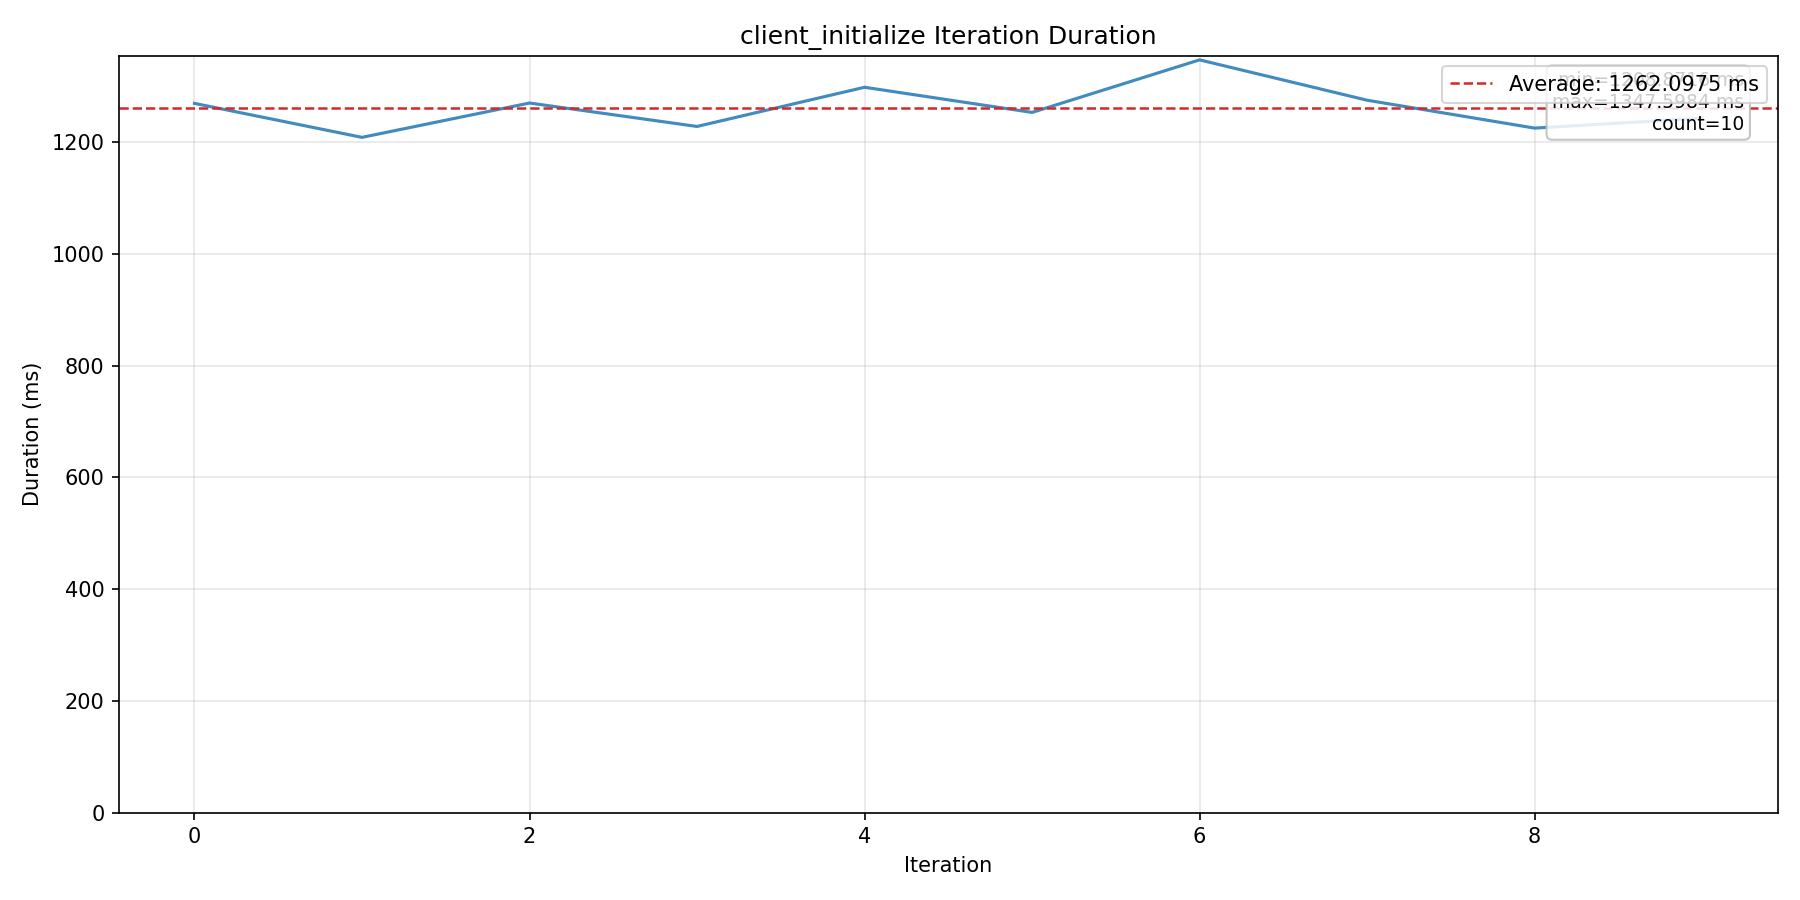
\includegraphics[width=0.48\linewidth]{images/client_initialize_before.png}
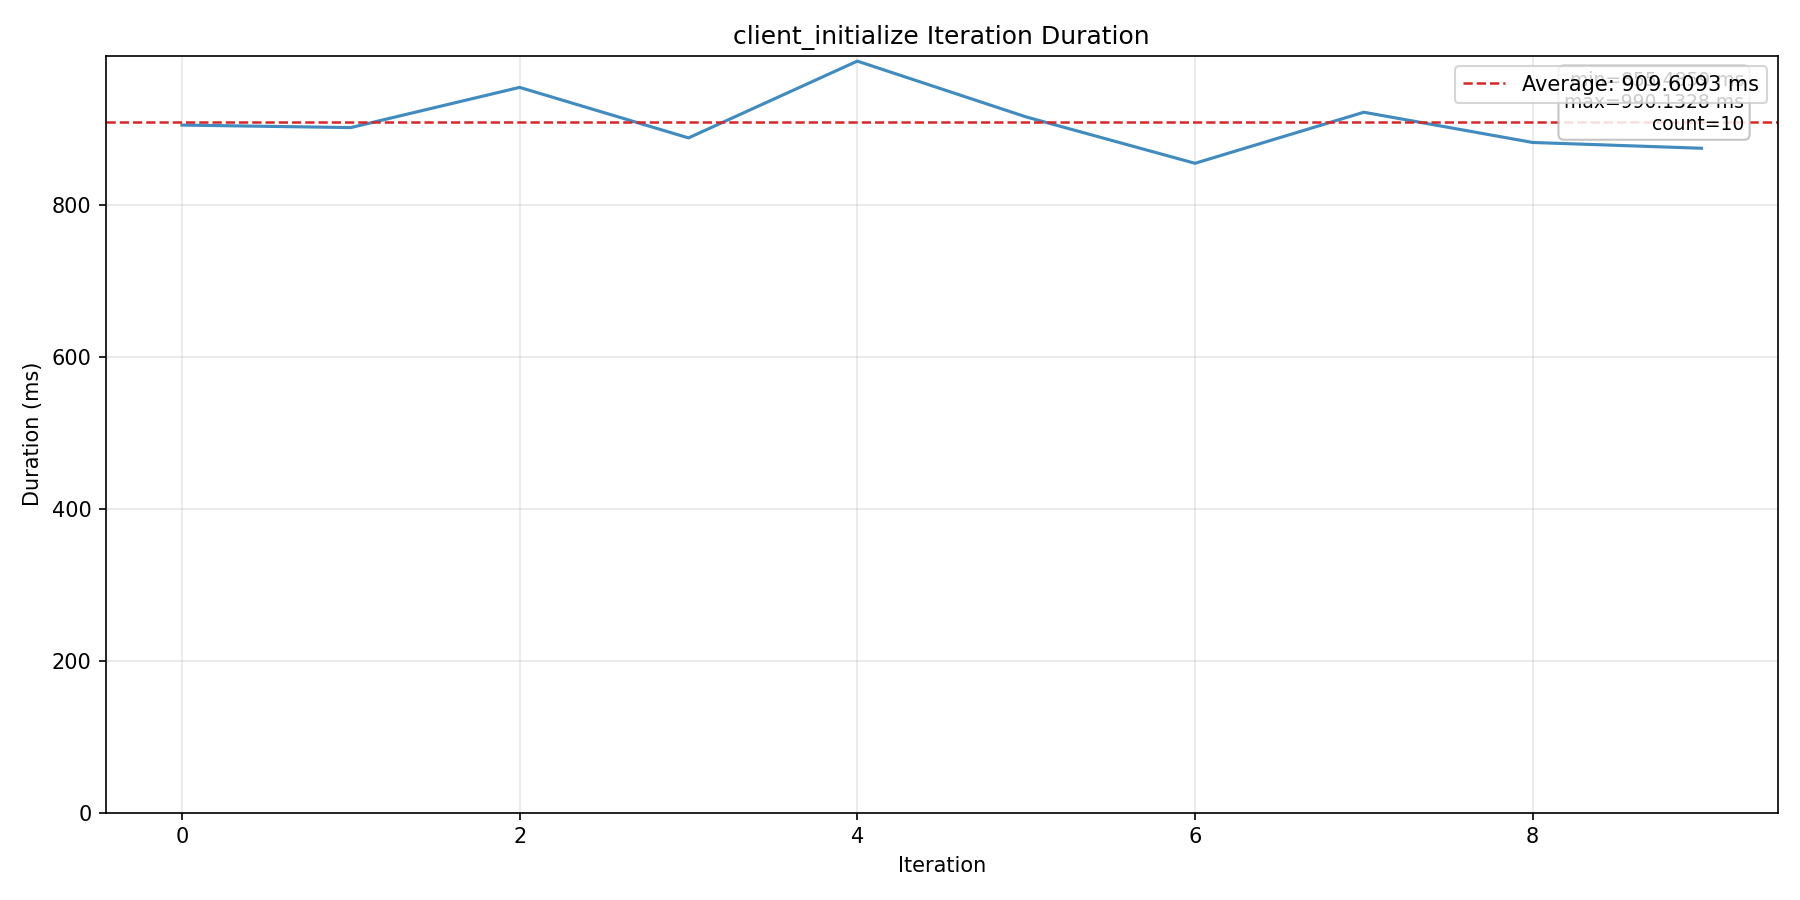
\includegraphics[width=0.48\linewidth]{images/client_initialize_after.png}
\caption{\texttt{client\_initialize}基准的单次迭代耗时对比。左图为优化前，右图为优化后。可以看到优化后整条曲线整体下移，平均值和峰值均明显降低。}
\label{fig:blockstate_compact_benchmark_curves}
\end{figure}

这一结果说明，状态系统优化不仅减少了静态内存占用，也直接改善了客户端启动阶段的状态容器构建、默认状态初始化以及依赖状态查询的资源预热路径。由于\texttt{client\_initialize}属于多个子系统共同参与的综合基准，单项数据结构重构仍能带来接近三成的整体耗时下降，说明状态对象曾经是初始化阶段的重要热点。

\textbf{优化前后对比总结}：表\ref{tab:blockstate_comparison}从多个维度对比了优化前后的设计差异。

\begin{table}[h]
\centering
\caption{方块状态系统优化前后设计对比}
\label{tab:blockstate_comparison}
\begin{tabular}{lcc}
\toprule
\textbf{维度} & \textbf{优化前} & \textbf{优化后} \\
\midrule
状态对象数据结构 & 每个状态持两张哈希表 & 紧凑的值索引数组 \\
状态切换方式 & 哈希表查找 + 跳转表访问 & O(1) 整数运算 + 数组访问 \\
内存布局 & 分散的堆对象 & 连续的一维数组 \\
单状态对象大小 & 约200+字节 & 约64字节 \\
状态容器构建 & 枚举 + 哈希匹配 & 按基数直接生成 \\
缓存友好性 & 差（指针跳转多） & 好（连续内存访问） \\
\bottomrule
\end{tabular}
\end{table}

这一重构的核心洞见是：如果状态空间可以表示为多维离散坐标，则所有状态可以按行主序映射到一维数组。每个状态只需存储其在数组中的索引，状态切换则退化为简单的整数运算——这比任何哈希表都更快、更紧凑。

\subsubsection{区块反序列化路径优化}

\textbf{背景：Minecraft 的区块同步是什么？}

对不熟悉 Minecraft 的读者来说，可以先把世界想象成一个巨大的三维数组。游戏不会一次性把整张世界地图都发给客户端，而是把世界拆成很多个 \emph{chunk} 逐块同步。一个 chunk 的大小是 $16 \times 256 \times 16$ 个方块，也就是一根竖直的 16x16 柱体，高度覆盖整个可玩世界。

如果直接把整个 chunk 当成一个整体处理，单次就要涉及 65536 个方块，数据量太大，所以 Minecraft 又把 chunk 在垂直方向切成 16 个 \emph{section}。每个 section 是 $16 \times 16 \times 16 = 4096$ 个方块，是网络同步和内部存储的更小粒度单元。这样做的好处是：只有某一段需要更新时，不必重发整根柱体。

\textbf{背景：一条 chunk 数据里都包含什么？}

客户端收到区块数据后，不只是把方块 ID 放回数组里这么简单，还要恢复成后续渲染、光照和碰撞系统都能直接使用的结构。这里面通常包含几类信息：

\begin{itemize}
    \item \textbf{chunk 坐标}：\texttt{x} / \texttt{z}，用于说明这块数据对应世界中的哪一列。
    \item \textbf{section mask}：16 位掩码，表示哪些垂直 section 实际存在。空 section 可以省略，不必全发。
    \item \textbf{heightmap}：一个 16x16 的高度图，记录每个 XZ 位置最高的非空气方块高度，供天空光照、地形轮廓和部分生成逻辑使用。
    \item \textbf{biomes}：4x4x4 的生物群系采样，用来决定草色、天空颜色、降雨表现等外观效果。
    \item \textbf{section 数据}：每个 section 里包含 4096 个方块状态 ID，以及天空光照和方块光照数组。
\end{itemize}

\textbf{为什么这条路径会慢？}

在网络同步路径中，\texttt{ChunkSerializer::deserializeChunk} 负责把服务端发送的整块区块数据还原成\texttt{ChunkData}。这条路径的特点不是纯计算，而是连续字节流解析、临时缓冲区分配和跨层数据搬运。优化前，函数会先把每个 section 读入临时\texttt{std::vector<u8>}，再逐项解析方块状态并拷贝光照数组；因此 \textit{wall duration} 主要消耗在内存搬运和容器重分配上，而不是函数本身的逻辑。

在 Perfetto 里，\textit{wall duration} 表示函数从进入到退出的总耗时，\textit{self duration} 表示扣掉子调用以后，函数自身真正消耗的时间。截图里优化前的 wall duration 大约在 0.4--0.7ms，而 self duration 只有个位数到十几微秒，这说明热点并不在“这层函数写了很多计算”，而在它触发的 section 解析、缓冲区拷贝和对象构建。

\textbf{优化思路}

Perfetto 追踪显示，\texttt{deserializeChunk} 的 wall duration 约 0.4--0.7\,ms，而 self duration 仅有十几微秒，说明瓶颈不在函数自身的计算逻辑，而在它触发的底层内存操作——临时堆分配、逐元素写入和重复拷贝。具体而言，优化前的代码存在三类问题：

\begin{enumerate}
    \item \textbf{冗余的临时缓冲区}：\texttt{readBytes()} 每次调用都 \texttt{new} 一个 \texttt{std::vector<u8>}，将字节流数据拷入其中，返回给调用方后再拷入最终目标。对于高度图（256\,B）、生物群系和每个 section 的数据，这意味着多一次堆分配加一次冗余拷贝。
    \item \textbf{逐元素写入}：序列化时，4096 个方块状态各用 4 次 \texttt{push\_back} 拼接到输出向量（共 16384 次 \texttt{push\_back}）；反序列化时，逐个读取 4 字节、移位拼合、再调用 \texttt{setBlockStateIdFast()}。每次 \texttt{push\_back} 都要检查容量、可能触发重分配；每次 \texttt{setBlockStateIdFast()} 还会额外执行方块计数和 tick 计数器的逐块更新。
    \item \textbf{序列化器增量增长}：\texttt{serializeChunk} 使用默认构造的 \texttt{PacketSerializer}，其内部 \texttt{std::vector<u8>} 容量从零开始，随着数据写入反复扩容，产生多次 \texttt{realloc} + \texttt{memcpy}。
\end{enumerate}

针对这三个瓶颈，优化采取了三组对应的策略：

\begin{enumerate}
    \item \textbf{零拷贝直写——以 \texttt{readBytesInto()} 替代 \texttt{readBytes()}}。

    原始的 \texttt{readBytes(size)} 在反序列化器内部构造 \texttt{std::vector<u8>}，用迭代器拷贝数据后按值返回；调用方再从临时向量中读取。新的 \texttt{readBytesInto(dest, size)} 直接将字节流 \texttt{memcpy} 到调用方提供的缓冲区，跳过堆分配和中间向量。具体应用：

    \begin{itemize}
        \item 高度图：用栈上 \texttt{std::array<u8, 256>} 接收，彻底消除堆分配。
        \item 生物群系：调用方预建好精确大小的 \texttt{std::vector<u8>}，\texttt{readBytesInto} 直写其中。
        \item Section 数据：同样预分配向量，直写后传给 \texttt{deserializeChunkSection()}。
    \end{itemize}

    \item \textbf{批量连续拷贝——以 \texttt{memcpy} 替代逐元素循环}。

    4096 个方块状态在内存中本质上是 $4096 \times 4 = 16384$ 字节的连续数据。在 little-endian 平台（覆盖所有现代 x86/ARM），其字节序与网络字节流一致，可以直接用一次 \texttt{memcpy} 完成整块搬移：

    \begin{itemize}
        \item \textbf{反序列化}：将原来的 4096 次循环（每次读 4 字节、移位、或运算、调用 \texttt{setBlockStateIdFast()}）替换为一次 \texttt{memcpy} 写入 \texttt{m\_blockStates}，并在结束后调用一次 \texttt{rebuildTickCounters()} 重建计数器。光照数据同理：直接 \texttt{resize} section 内部向量后 \texttt{memcpy}，不再构造临时向量再移动构造 \texttt{NibbleArray}。
        \item \textbf{序列化}：将 4096$\times$4 次 \texttt{push\_back} 替换为一次 \texttt{memcpy}。输出缓冲区使用精确大小的 \texttt{std::vector<u8>(SECTION\_DATA\_SIZE)} 构造（而非 \texttt{reserve} + 反复 \texttt{push\_back}），配合裸指针 \texttt{u8* out} 顺序写入：先写 2 字节 \texttt{blockCount}，再 \texttt{memcpy} 方块状态（16\,KB），再 \texttt{memcpy} 两个光照数组。总写入次数从 16384+ 次 \texttt{push\_back} 降至 3 次 \texttt{memcpy} + 2 次指针写入。
    \end{itemize}

    非little-endian平台保留逐字节回退路径，由编译期 \texttt{\#if} 切换。

    \item \textbf{精确预分配——一次性确定缓冲区容量}。

    \texttt{serializeChunk} 在构造 \texttt{PacketSerializer} 前先遍历各 section 计算精确字节大小，然后传入 \texttt{PacketSerializer(expectedSize)}，内部一次 \texttt{reserve} 即可容纳整包数据，消除了增量扩容带来的多次 \texttt{realloc}。高度图的序列化也从 256 次 \texttt{writeU8} 改为先填入栈上 \texttt{std::array}、再单次 \texttt{writeBytes} 批量写入。
\end{enumerate}

整体而言，这三组策略的核心逻辑是一致的：\textbf{将"逐元素写入 + 中间缓冲区"的模式替换为"预分配 + 连续拷贝"的模式}。这在内存密集型路径上尤为有效——减少了堆分配次数（每次 \texttt{new} 都涉及内核态切换或锁竞争）、消除了冗余数据拷贝、改善了缓存局部性（连续 \texttt{memcpy} 对 prefetcher 友好），同时将逐块维护的计数器更新分摊为一次批量重建。

\begin{figure}[h]
\centering
\begin{minipage}[t]{0.48\linewidth}
\centering
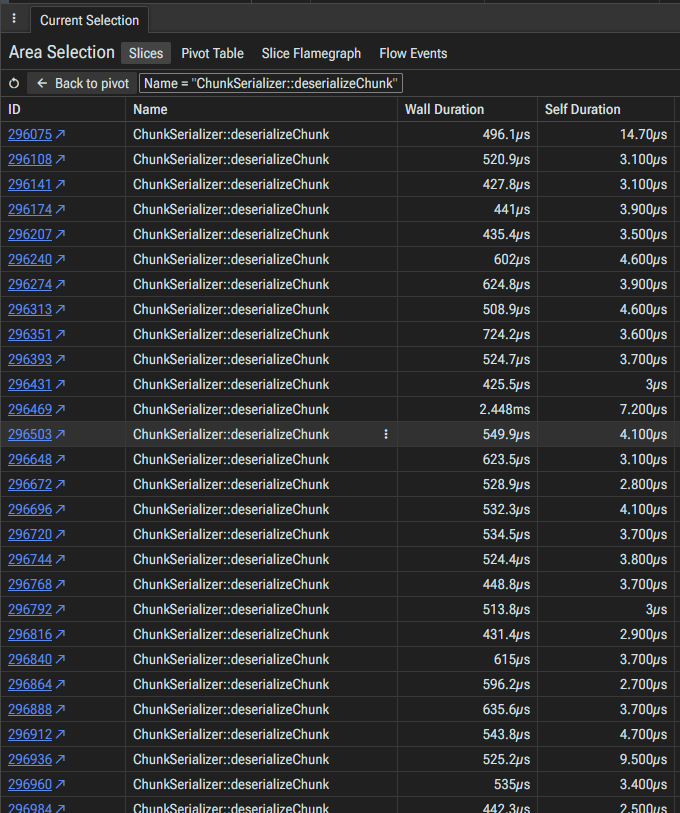
\includegraphics[width=\linewidth]{images/chunkdeser_before.png}
\par\small 优化前
\end{minipage}
\hfill
\begin{minipage}[t]{0.48\linewidth}
\centering
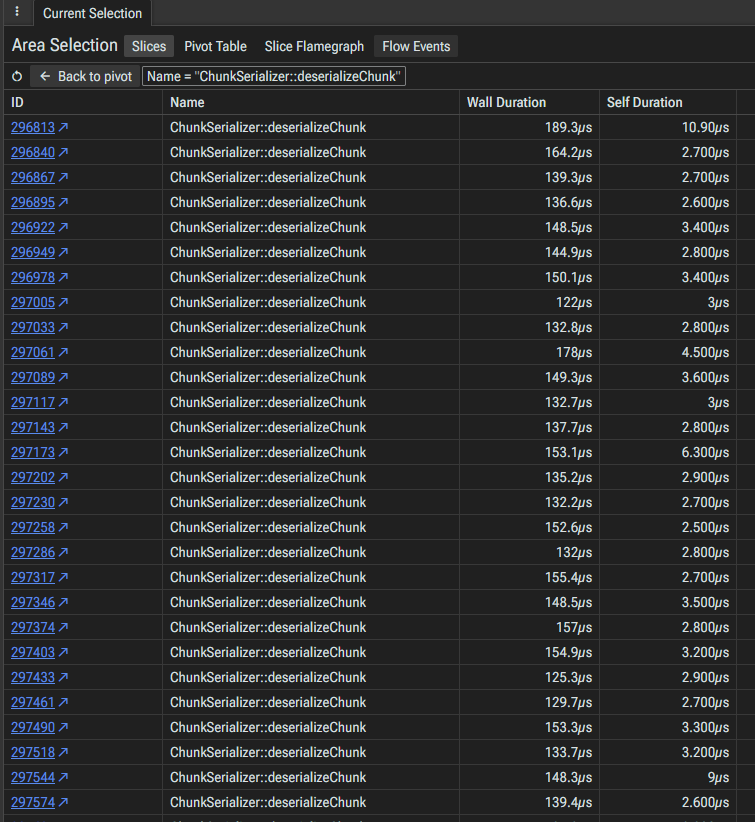
\includegraphics[width=\linewidth]{images/chunkdeser_after.png}
\par\small 优化后
\end{minipage}
\caption{\texttt{ChunkSerializer::deserializeChunk} 的 Perfetto 对比。左图为优化前，右图为优化后。可以看到 wall duration 由约0.4--0.7ms降至约0.12--0.19ms，而 self duration 始终只有个位数到十几微秒，说明主要收益来自削减临时缓冲区和逐段解析带来的内存开销。}
\label{fig:chunkdeserialize_compare}
\end{figure}

\textbf{结果解读}：优化后 \texttt{deserializeChunk} 的 wall duration 由约 0.4--0.7\,ms 降至约 0.12--0.19\,ms，降幅约 70\%。self duration 基本不变，印证了收益来自更少的堆分配和更连续的内存访问模式，而非指令级别的优化。这符合内存带宽受限路径的典型特征：减少拷贝次数和改善局部性的收益远大于减少算术运算。

\subsubsection{内存对齐}

在Vulkan渲染相关代码中大量使用\texttt{alignas}确保GPU缓冲区的内存对齐：

Uniform缓冲区结构体对齐要求严格：\texttt{vec4}需要16字节对齐，标量通常需要4字节对齐。正确的对齐避免了GPU读取时的性能惩罚和潜在的渲染错误。

\subsection{模板元编程}

\subsubsection{类型安全容器}

\texttt{EnumSet<E>}模板类提供类型安全的枚举集合，使用\texttt{static\_assert}在编译期验证模板参数是枚举类型，并提供\texttt{forEach}方法遍历所有设置的枚举值。

\subsubsection{Result<T>错误处理}

\texttt{Result<T>}模板类实现了类型安全的错误处理，通过模板特化支持\texttt{Result<void>}和\texttt{Result<unique\_ptr<T>>}等特殊情况。使用SFINAE约束构造函数，防止隐式转换导致的意外行为。

\subsubsection{序列化模板}

网络数据包序列化使用模板函数\texttt{writeInteger<T>}，根据类型大小选择不同的序列化方式，编译期确定分支，无运行时开销。

\subsection{多线程与并发}

\subsubsection{原子操作与内存序}

项目正确使用了原子操作和内存序：

\textbf{memory\_order\_acquire}：读取操作，确保后续操作不会重排到此操作之前。

\textbf{memory\_order\_release}：写入操作，确保之前的操作不会重排到此操作之后。

\textbf{协作取消}：取消令牌使用原子布尔，任务执行时使用acquire语义读取，设置取消时使用release语义写入。

\subsubsection{线程安全容器}

线程池使用\texttt{std::priority\_queue}配合\texttt{std::mutex}和\texttt{std::condition\_variable}实现任务队列。高优先级任务先执行，同优先级按提交时间排序。

\subsubsection{异步操作}

\texttt{std::future}/\texttt{std::promise}用于异步区块加载。调用方通过\texttt{future}获取结果，实现线程在等待结果的同时执行其他工作。

\subsection{性能编码技巧}

\subsubsection{内联函数}

项目有412处使用\texttt{inline}，主要用于头文件中的小型函数。编译器会根据函数复杂度和调用频率决定是否内联。热点函数（如数学运算、坐标转换）内联后消除了函数调用开销。

\subsubsection{缓存友好设计}

\textbf{数据布局}：光照引擎使用紧凑的64位编码将坐标、等级、方向打包到单个整数，提高缓存利用率。

\textbf{状态布局}：方块状态系统采用“属性布局表 + 值索引数组 + stride寻址”设计，将状态切换转化为整数运算。相比基于哈希表的表示，这种布局更加连续，适合大量只读访问和频繁状态跳转的工作负载。

\textbf{预分配缓存}：线程池预分配任务缓存，避免频繁内存分配。

\textbf{局部性优化}：区块生成时按Z字形顺序访问相邻区块，提高缓存命中率。

\subsubsection{分支预测优化}

在热点代码中使用\texttt{[[likely]]}和\texttt{[[unlikely]]}属性提示编译器分支概率。例如，在错误处理分支使用\texttt{[[unlikely]]}，让编译器将错误处理代码放在冷代码区域。

\subsection{类型系统}

项目定义了清晰的类型别名系统，避免魔法数字和提高可读性：

基本类型别名：\texttt{i8, i16, i32, i64, u8, u16, u32, u64, f32, f64}。

游戏类型别名：\texttt{ChunkCoord, BlockCoord, EntityId, ItemId, BiomeId, PlayerId}。

类型别名配合\texttt{static\_assert}确保类型大小符合预期，如\texttt{static\_assert(sizeof(f32) == 4)}。

\subsection{总结}

\begin{table}[h]
\centering
\caption{现代C++特性使用统计}
\label{tab:cpp_features}
\begin{tabular}{lc}
\toprule
\textbf{特性} & \textbf{使用次数} \\
\midrule
constexpr & 2926+ \\
auto & 11543+ \\
Lambda表达式 & 4235+ \\
std::move/forward & 2068+ \\
if constexpr & 35+ \\
std::optional & 367+ \\
模板 & 620+ \\
智能指针 & 5832+ \\
STL容器 & 4217+ \\
\bottomrule
\end{tabular}
\end{table}

通过充分利用C++20特性和现代编译器优化，项目在保持代码可读性和类型安全的同时，实现了高性能游戏引擎所需的基础设施。编译期计算将运行时开销转移到编译时，智能指针确保内存安全，原子操作保证线程安全，模板元编程实现类型安全的泛型代码，而状态系统紧凑化则进一步说明：性能优化不仅来自编译器选项，也来自对核心数据结构的持续重构与压缩。在本项目中，这种数据结构级别的优化已经通过基准测试反映为27.93\%的客户端初始化耗时下降和1.39倍的吞吐提升。
